\documentclass[aspectratio=169,11pt]{beamer}

\def\courseTitle{Industrial Security (Bachelor)}
\def\courseSubtitle{Section 05 -- Threat Landscape}
\def\sectionNumber{05}
\def\sectionTitle{Threat Landscape}

% =====================================================================
% Industrial Security lecture series -- modern Beamer preamble.
%
% Each slide deck must define the following BEFORE \input{}-ing this:
%   \def\courseTitle{...}        e.g. Industrial Security (Bachelor)
%   \def\courseSubtitle{...}     e.g. Section 3 -- Network Architecture
%   \def\sectionNumber{...}      e.g. 03
%   \def\sectionTitle{...}       e.g. Industrial Network Architectures
%
% Optional:
%   \def\courseAuthor{...}       defaults to "Lecture Notes"
%   \def\courseInstitute{...}    defaults to "Department of Computer Science"
%   \def\companyLogo{...}        path to a logo image (PDF/PNG/JPG).
%
% Callout macros (use anywhere inside a frame):
%   \begin{notebox}{title}      ... \end{notebox}
%   \begin{importantbox}{title} ... \end{importantbox}
%   \begin{warningbox}{title}   ... \end{warningbox}
%   \begin{tipbox}{title}       ... \end{tipbox}
%   \begin{defbox}{title}       ... \end{defbox}
%   \begin{takeawaybox}{title}  ... \end{takeawaybox}
%   \begin{quotebox}            ... \end{quotebox}
% =====================================================================

% --- Speaker-notes mode (toggled by Makefile via -usepretex) ----------
% When notesmode=1, build a side-by-side slide+notes PDF for the
% lecturer. When unset/0, build the clean slides-only PDF.
\providecommand{\notesmode}{0}
\ifnum\notesmode=1
  \usepackage{pgfpages}
  \setbeameroption{show notes on second screen=right}
  \setbeamerfont{note page}{size=\small}
\fi

\usepackage[utf8]{inputenc}
\usepackage[T1]{fontenc}
\usepackage[english]{babel}
% Modern type pair: IBM Plex Sans for text, IBM Plex Mono for code.
% Math stays in lmodern; Plex is the dominant family on every text frame.
\usepackage{plex-sans}
\usepackage{plex-mono}
\renewcommand{\familydefault}{\sfdefault}
\usepackage[activate={true,nocompatibility},final,tracking=true,kerning=true,spacing=true,factor=1100,stretch=10,shrink=10]{microtype}
\usepackage{graphicx}
\usepackage{listings}
\usepackage{xcolor}
\usepackage{colortbl}
\usepackage{tikz}
\usepackage{booktabs}
\usepackage{array}
\usepackage{hyperref}
\usepackage{amsmath}
\usepackage{amssymb}
\usepackage{tcolorbox}
\tcbuselibrary{skins, breakable, raster}
\usepackage{fontawesome5}

% =====================================================================
% Shared TikZ styles for the Industrial Security lecture series.
% Loaded by every slide deck and exercise sheet that uses TikZ.
% =====================================================================

\usetikzlibrary{
  arrows.meta,
  shapes,
  shapes.geometric,
  shapes.symbols,
  shapes.multipart,
  positioning,
  fit,
  calc,
  backgrounds,
  decorations.pathmorphing,
  decorations.pathreplacing,
  decorations.text,
  patterns,
  matrix,
  shadows
}

% --- colour palette --------------------------------------------------
\definecolor{isOT}{HTML}{1F4E79}     % OT (deep blue)
\definecolor{isIT}{HTML}{6F2DA8}     % IT (purple)
\definecolor{isSafety}{HTML}{C00000} % safety red
\definecolor{isNet}{HTML}{2E7D32}    % network green
\definecolor{isAttack}{HTML}{B23A48} % attack red
\definecolor{isAccent}{HTML}{E08E0B} % amber
\definecolor{isMute}{HTML}{6B6B6B}   % grey
\definecolor{isLight}{HTML}{EDF2F8}  % light background
\definecolor{isPLC}{HTML}{2C5282}
\definecolor{isHMI}{HTML}{2F855A}
\definecolor{isSCADA}{HTML}{6B46C1}

% --- generic node styles --------------------------------------------
\tikzset{
  isnode/.style={
    draw, rounded corners=2pt, minimum height=8mm, minimum width=18mm,
    font=\small, align=center, thick
  },
  isbox/.style={isnode, fill=isLight},
  plc/.style={isnode, fill=isPLC!15, draw=isPLC, thick},
  hmi/.style={isnode, fill=isHMI!15, draw=isHMI, thick},
  scada/.style={isnode, fill=isSCADA!15, draw=isSCADA, thick},
  sensor/.style={isnode, fill=isNet!10, draw=isNet, minimum height=6mm, minimum width=14mm, font=\scriptsize},
  actuator/.style={isnode, fill=isAccent!15, draw=isAccent, minimum height=6mm, minimum width=14mm, font=\scriptsize},
  firewall/.style={isnode, fill=isAttack!15, draw=isAttack, thick},
  server/.style={isnode, fill=isMute!15, draw=isMute!80, thick},
  switch/.style={isnode, fill=isLight, draw=black!60, minimum height=6mm, minimum width=14mm, font=\scriptsize},
  workstation/.style={isnode, fill=white, draw=isOT, thick},
  attacker/.style={isnode, fill=isAttack!20, draw=isAttack, thick, font=\small\bfseries},
  inetnode/.style={draw, ellipse, minimum width=24mm, minimum height=10mm, font=\scriptsize, fill=isLight, thick},
  process/.style={isnode, fill=isOT!15, draw=isOT, thick, minimum width=24mm},
  zone/.style={
    draw, rounded corners=4pt, thick, dashed, inner sep=4mm
  },
  conduit/.style={-{Stealth[length=2.5mm]}, thick, isNet!80!black},
  attack/.style={-{Stealth[length=2.5mm]}, thick, isAttack, dashed},
  flow/.style={-{Stealth[length=2.5mm]}, thick, isOT!70!black},
  netline/.style={thick, black!60},
  axisline/.style={-{Stealth[length=2mm]}, thick, black!70},
  tag/.style={font=\scriptsize\itshape, fill=white, inner sep=1pt},
  level/.style={
    draw, fill=isLight, minimum width=0.85\linewidth, minimum height=8mm,
    font=\small, anchor=west
  },
  brace/.style={decorate, decoration={brace, amplitude=4pt, raise=2pt}},
  legendbox/.style={draw, rounded corners=2pt, fill=isLight, inner sep=2mm, font=\scriptsize, align=left}
}

% --- handy macros ----------------------------------------------------
% \plcicon, \hmiicon etc as simple labelled boxes; useful inline.
\newcommand{\plcicon}[1][PLC]{\tikz[baseline=-0.6ex]{\node[plc, minimum width=10mm, minimum height=5mm, font=\scriptsize, inner sep=1pt]{#1};}}
\newcommand{\hmiicon}[1][HMI]{\tikz[baseline=-0.6ex]{\node[hmi, minimum width=10mm, minimum height=5mm, font=\scriptsize, inner sep=1pt]{#1};}}
\newcommand{\fwicon}[1][FW]{\tikz[baseline=-0.6ex]{\node[firewall, minimum width=10mm, minimum height=5mm, font=\scriptsize, inner sep=1pt]{#1};}}


\graphicspath{{.}{../../../template/}}

% --- defaults --------------------------------------------------------
\providecommand{\courseAuthor}{Lecture Notes}
\providecommand{\courseInstitute}{Department of Computer Science}
\providecommand{\companyLogo}{logo}

% --- modern palette --------------------------------------------------
\definecolor{slideAccent}{HTML}{1F4E79}       % primary navy
\definecolor{slideSecondary}{HTML}{E08E0B}    % amber accent

% --- Corporate branding overrides ------------------------------------
% A user-editable `branding.tex` at the repo root can override the
% logo path, author/institute lines, and brand colours. If the file is
% missing the built-in defaults above stay in effect.
\IfFileExists{../../../branding.tex}{% =====================================================================
% Corporate / institutional branding -- single file to customise the
% look of the entire course (slides, notes, exercises, labs).
%
% HOW TO REBRAND IN UNDER A MINUTE:
%   1. Replace `branding/logo.pdf` with your own logo
%      (PDF preferred; PNG and JPG also work -- name it `logo.<ext>`).
%   2. (Optional) change the two colours below to your brand palette.
%   3. (Optional) override the author/institute lines below.
%   4. Re-run `make` at the repo root. That's it.
%
% Everything in this file has sensible defaults; you can delete a line
% to fall back to the built-in defaults, or comment it out.
%
% This file is loaded automatically by the slides, exercise, and lab
% preambles -- you never need to \input it manually.
% =====================================================================

% --- Logo --------------------------------------------------------------
% Path is resolved from each leaf-build directory; the default points at
% the shared `branding/` folder at the repo root. If you put your logo
% somewhere else, set the full or relative path here (without extension):
\renewcommand{\companyLogo}{../../../branding/logo}

% --- Author / institute (appears on the title page footer) ------------
\renewcommand{\courseAuthor}{}
\renewcommand{\courseInstitute}{}

% --- Brand colours ----------------------------------------------------
% slideAccent      = primary brand colour (title bands, accent rule)
% slideSecondary   = secondary brand colour (section badge, highlight)
% Both use HTML hex codes. Keep enough contrast against white text.
\definecolor{slideAccent}{HTML}{00205B}      % deep navy
\definecolor{slideSecondary}{HTML}{00A0DC}   % light blue accent
}{}
\definecolor{slideTitle}{HTML}{0F2A44}        % near-black navy
\definecolor{slideMuted}{HTML}{6B6B6B}
\definecolor{slideBg}{HTML}{FFFFFF}
\definecolor{slidePanel}{HTML}{F4F7FB}
\definecolor{slideRule}{HTML}{D6DEE8}

% Callout colours
\definecolor{calNote}{HTML}{1F4E79}
\definecolor{calImportant}{HTML}{B23A48}
\definecolor{calWarning}{HTML}{C77700}
\definecolor{calTip}{HTML}{2E7D32}
\definecolor{calDef}{HTML}{6B46C1}
\definecolor{calTake}{HTML}{0F2A44}

% --- beamer theme ---------------------------------------------------
\useinnertheme{rectangles}
\usefonttheme{professionalfonts}

\setbeamertemplate{navigation symbols}{}
\setbeamertemplate{itemize items}[circle]
\setbeamertemplate{enumerate items}[default]
\setbeamertemplate{section in toc}[ball numbered]
\setbeamercolor{section in toc}{fg=slideTitle}

% Colours
\setbeamercolor{normal text}{fg=slideTitle, bg=slideBg}
\setbeamercolor{title}{fg=slideAccent}
\setbeamercolor{subtitle}{fg=slideMuted}
\setbeamercolor{frametitle}{fg=slideAccent}
\setbeamercolor{structure}{fg=slideAccent}
\setbeamercolor{itemize item}{fg=slideAccent}
\setbeamercolor{itemize subitem}{fg=slideSecondary}
\setbeamercolor{block title}{fg=white, bg=slideAccent}
\setbeamercolor{block body}{fg=slideTitle, bg=slidePanel}
\setbeamercolor{alerted text}{fg=slideSecondary}

% Fonts
\setbeamerfont{title}{series=\bfseries, size=\Large}
\setbeamerfont{subtitle}{series=\mdseries, size=\normalsize}
\setbeamerfont{frametitle}{series=\bfseries, size=\large}
\setbeamerfont{block title}{series=\bfseries, size=\normalsize}
\setbeamerfont{footline}{size=\tiny}

% --- frametitle: title bar + accent underline + section badge -------
% The accent rules are wrapped in a zero-width box so they never
% contribute to the surrounding hbox width (no Overfull warnings).
\setbeamertemplate{frametitle}{%
  \nointerlineskip
  \begin{beamercolorbox}[wd=\paperwidth, ht=2.8ex, dp=1.6ex, leftskip=1.2em, rightskip=1.2em]{frametitle}%
    \usebeamerfont{frametitle}\insertframetitle%
    \hfill
    {\color{slideMuted}\small \sectionNumber}%
  \end{beamercolorbox}%
  \nointerlineskip
  \makebox[0pt][l]{\hspace*{1.2em}\textcolor{slideSecondary}{\rule{2.5em}{1pt}}\textcolor{slideAccent}{\rule{\dimexpr\paperwidth-3.7em\relax}{1pt}}}%
  \par\vskip4pt
}

% --- footer ---------------------------------------------------------
\defbeamertemplate*{footline}{is-footer}{%
  \leavevmode%
  \hbox{%
    \begin{beamercolorbox}[wd=.55\paperwidth, ht=2.4ex, dp=1ex, leftskip=1em]{author in head/foot}%
      {\color{slideMuted}\tiny \courseTitle{} \;\; $\bullet$ \;\; Section \sectionNumber{} -- \sectionTitle}%
    \end{beamercolorbox}%
    \begin{beamercolorbox}[wd=.45\paperwidth, ht=2.4ex, dp=1ex, rightskip=1em]{title in head/foot}%
      \hfill {\color{slideMuted}\tiny \insertframenumber{} / \inserttotalframenumber}%
    \end{beamercolorbox}%
  }%
  \vskip2pt
}

% --- listings -------------------------------------------------------
\definecolor{codebg}{HTML}{F4F7FB}
\definecolor{codekw}{HTML}{0F2A44}
\definecolor{codestr}{HTML}{8B3A3A}
\definecolor{codecom}{HTML}{5A7D54}

\lstset{
    backgroundcolor=\color{codebg},
    basicstyle=\ttfamily\scriptsize\color{slideTitle},
    keywordstyle=\color{codekw}\bfseries,
    stringstyle=\color{codestr},
    commentstyle=\color{codecom}\itshape,
    breaklines=true,
    frame=leftline,
    framerule=2pt,
    rulecolor=\color{slideAccent},
    numbers=left,
    numberstyle=\tiny\color{slideMuted},
    numbersep=8pt,
    showstringspaces=false,
    tabsize=2,
    captionpos=b,
    xleftmargin=0.6em
}

% --- callout boxes --------------------------------------------------
% Shared base style for all callout boxes.
% Subtle drop shadow gives the boxes a hint of elevation without distraction.
\tcbset{
  isCallout/.style={
    enhanced, breakable, sharp corners=northeast,
    arc=2pt, boxrule=0pt,
    leftrule=3pt,
    fonttitle=\bfseries\small,
    coltitle=white,
    fontupper=\small,
    left=2mm, right=2mm, top=1.5mm, bottom=1.5mm,
    drop fuzzy shadow=black!30,
    title={#1}
  }
}

\newtcolorbox{notebox}[1]{
  isCallout={#1},
  colback=calNote!8, colframe=calNote, leftrule=3pt,
  colbacktitle=calNote, attach boxed title to top left={xshift=2mm, yshift=-1.2mm},
  boxed title style={colback=calNote, arc=1pt, boxrule=0pt, left=2mm, right=2mm, top=0.5mm, bottom=0.5mm}
}

\newtcolorbox{importantbox}[1]{
  isCallout={#1},
  colback=calImportant!7, colframe=calImportant, leftrule=4pt,
  colbacktitle=calImportant, attach boxed title to top left={xshift=2mm, yshift=-1.2mm},
  boxed title style={colback=calImportant, arc=1pt, boxrule=0pt, left=2mm, right=2mm, top=0.5mm, bottom=0.5mm}
}

\newtcolorbox{warningbox}[1]{
  isCallout={#1},
  colback=calWarning!10, colframe=calWarning, leftrule=4pt,
  colbacktitle=calWarning, attach boxed title to top left={xshift=2mm, yshift=-1.2mm},
  boxed title style={colback=calWarning, arc=1pt, boxrule=0pt, left=2mm, right=2mm, top=0.5mm, bottom=0.5mm}
}

% Alias warnbox = warningbox, with an optional title (default = "Caution")
\newtcolorbox{warnbox}[1][Caution]{
  isCallout={#1},
  colback=calWarning!10, colframe=calWarning, leftrule=4pt,
  colbacktitle=calWarning, attach boxed title to top left={xshift=2mm, yshift=-1.2mm},
  boxed title style={colback=calWarning, arc=1pt, boxrule=0pt, left=2mm, right=2mm, top=0.5mm, bottom=0.5mm}
}

\newtcolorbox{tipbox}[1]{
  isCallout={#1},
  colback=calTip!8, colframe=calTip, leftrule=3pt,
  colbacktitle=calTip, attach boxed title to top left={xshift=2mm, yshift=-1.2mm},
  boxed title style={colback=calTip, arc=1pt, boxrule=0pt, left=2mm, right=2mm, top=0.5mm, bottom=0.5mm}
}

\newtcolorbox{defbox}[1]{
  isCallout={#1},
  colback=calDef!8, colframe=calDef, leftrule=3pt,
  colbacktitle=calDef, attach boxed title to top left={xshift=2mm, yshift=-1.2mm},
  boxed title style={colback=calDef, arc=1pt, boxrule=0pt, left=2mm, right=2mm, top=0.5mm, bottom=0.5mm}
}

\newtcolorbox{takeawaybox}[1]{
  enhanced, breakable, arc=3pt, boxrule=0pt,
  colback=calTake!7, colframe=calTake,
  toptitle=2mm, bottomtitle=2mm,
  fonttitle=\bfseries\normalsize, coltitle=white,
  colbacktitle=calTake,
  fontupper=\small,
  title={\faStar~Key Takeaway: #1},
  left=3mm, right=3mm, top=2mm, bottom=2mm
}

\newtcolorbox{quotebox}{
  enhanced, breakable, arc=2pt, boxrule=0pt,
  colback=slidePanel, colframe=slideMuted,
  leftrule=3pt, top=2mm, bottom=2mm, left=3mm, right=3mm,
  fontupper=\itshape\small,
}

% Convenience: inline highlight badge
\newcommand{\remembertag}{\tikz[baseline=-0.7ex]\node[fill=calImportant, text=white, font=\scriptsize\bfseries, rounded corners=2pt, inner sep=2pt]{REMEMBER};}
\newcommand{\tldr}{\tikz[baseline=-0.7ex]\node[fill=calTake, text=white, font=\scriptsize\bfseries, rounded corners=2pt, inner sep=2pt]{TL;DR};}

% Source attribution: tiny grey line, anchored bottom-left of the content area
% Usage:  \source{Symantec, \emph{W32.Stuxnet Dossier} v1.4, 2011.}
% Multiple sources:  \source{X.\ Y., 2018; Z, 2020.}
\newcommand{\source}[1]{%
  \par\nointerlineskip\vspace{0.4mm}%
  {\color{slideMuted}\fontsize{5.5}{6.5}\selectfont\textit{Source:} #1\par}%
}

% References slide: aggregate citations + further reading at the end of a section.
% Usage:  \referencesframe{ \item ... \item ... }
% The `frame` environment must be written literally in the deck, so this is a
% macro rather than a wrapper environment (beamer collects the frame body and
% trips over \newenvironment wrappers).
%
% allowframebreakstemplate=\insertcontinuationcount silences the trailing roman
% numeral when content fits on a single page.
\setbeamertemplate{frametitle continuation}[from second]
\newcommand{\referencesframe}[1]{%
  \begin{frame}[allowframebreaks]{References -- Section \sectionNumber}
    \fontsize{7.5}{9}\selectfont
    \setlength{\itemsep}{1pt}
    \begin{itemize}#1\end{itemize}
  \end{frame}%
}

% --- title page -----------------------------------------------------
\title[\courseTitle]{\courseTitle}
\subtitle{\courseSubtitle}
\author{\courseAuthor}
\institute{\courseInstitute}
\date{}

% Logo lookup: try the section directory, then the shared template/.
\newcommand{\showlogo}[1][2cm]{%
  \IfFileExists{\companyLogo.pdf}{\includegraphics[width=#1]{\companyLogo}}{%
    \IfFileExists{\companyLogo.png}{\includegraphics[width=#1]{\companyLogo}}{%
      \IfFileExists{\companyLogo.jpg}{\includegraphics[width=#1]{\companyLogo}}{%
        \IfFileExists{../../../template/\companyLogo.pdf}{\includegraphics[width=#1]{../../../template/\companyLogo}}{%
          \rule{0pt}{0pt}}}}}}

\setbeamertemplate{title page}{%
  \begin{tikzpicture}[remember picture, overlay]
    % accent band (taller to fit wrapped titles)
    \fill[slideAccent] (current page.north west) rectangle ([yshift=-3.4cm]current page.north east);
    \fill[slideSecondary] ([yshift=-3.4cm]current page.north west) rectangle ([yshift=-3.55cm]current page.north east);
    % section badge
    \node[fill=slideSecondary, text=white, font=\bfseries\normalsize, rounded corners=3pt, inner sep=4pt, anchor=north west]
      at ([xshift=1.2cm, yshift=-0.7cm]current page.north west) {Section \sectionNumber};
    % Course title (wraps if long)
    \node[anchor=north west, text=white, font=\bfseries\Large, align=left, text width=11cm]
      at ([xshift=1.2cm, yshift=-1.5cm]current page.north west) {\courseTitle};
    % Subtitle (wraps; smaller, separated)
    \node[anchor=north west, text=white, font=\mdseries\small, align=left, text width=11cm]
      at ([xshift=1.2cm, yshift=-2.7cm]current page.north west) {\courseSubtitle};
    \node[anchor=north east] at ([xshift=-1.2cm, yshift=-1.0cm]current page.north east)
      {\showlogo[2cm]};
    \node[anchor=south west, text=slideMuted, font=\small, align=left, text width=11cm]
      at ([xshift=1.2cm, yshift=1.0cm]current page.south west)
      {\textbf{\sectionTitle}\\[2pt]\textit{\courseAuthor}\\{\scriptsize\courseInstitute}};
  \end{tikzpicture}
}

% --- helper macros --------------------------------------------------
\newcommand{\learningobjectives}[1]{%
  \begin{frame}{Learning Objectives}
    \begin{tipbox}{\faGraduationCap~By the end of this section you will be able to}
      \begin{itemize}\setlength{\itemsep}{2pt}#1\end{itemize}
    \end{tipbox}
  \end{frame}}

\newcommand{\sectionoverviewframe}{%
  \begin{frame}[plain,noframenumbering]
    \titlepage
  \end{frame}
  \begin{frame}{Outline -- Section \sectionNumber}
    \tableofcontents
  \end{frame}}

\AtBeginSection[]{%
  \begin{frame}[plain,noframenumbering]
    \begin{tikzpicture}[remember picture, overlay]
      \fill[slideAccent] (current page.north west) rectangle (current page.south east);
      \fill[slideSecondary] ([yshift=-1pt]current page.center -| current page.west)
                            rectangle ([yshift=1pt]current page.center -| current page.east);
      \node[text=white, font=\scriptsize, anchor=south west]
        at ([xshift=1.2cm, yshift=1.0cm]current page.south west)
        {Section \sectionNumber{} -- \sectionTitle};
      \node[text=slideSecondary, font=\bfseries\Huge, anchor=south]
        at ([yshift=0.4cm]current page.center)
        {\thesection};
      \node[text=white, font=\bfseries\LARGE, align=center, anchor=north, text width=12cm]
        at ([yshift=-0.6cm]current page.center)
        {\insertsection};
    \end{tikzpicture}
  \end{frame}}

\newcommand{\closingframe}{%
  \begin{frame}[plain,noframenumbering]
    \begin{tikzpicture}[remember picture, overlay]
      \fill[slideAccent] (current page.north west) rectangle (current page.south east);
      \node[text=white, font=\bfseries\Huge, anchor=center, align=center, text width=14cm]
        at ([yshift=8mm]current page.center) {End of Section \sectionNumber};
      \fill[slideSecondary] ([xshift=-1.5cm, yshift=-4mm]current page.center)
                            rectangle ([xshift=1.5cm, yshift=-6mm]current page.center);
      \node[text=white, font=\large, anchor=north, align=center, text width=14cm]
        at ([yshift=-1.2cm]current page.center) {\sectionTitle};
      \node[text=slideSecondary, font=\normalsize, anchor=south] at ([yshift=1.2cm]current page.south) {Questions and discussion};
      \node[anchor=south east] at ([xshift=-1cm, yshift=1cm]current page.south east) {\showlogo[1.5cm]};
    \end{tikzpicture}
  \end{frame}}


\begin{document}

\sectionoverviewframe

\learningobjectives{
  \item Categorise threat actors targeting industrial environments.
  \item Map ICS attacks to the MITRE ATT\&CK for ICS matrix.
  \item Analyse landmark incidents: Stuxnet, Ukraine, TRITON, Colonial.
  \item Identify supply-chain and insider risk vectors.
}

\section{Threat Actors and Frameworks}

\begin{frame}{Threat Actor Categories}
\centering
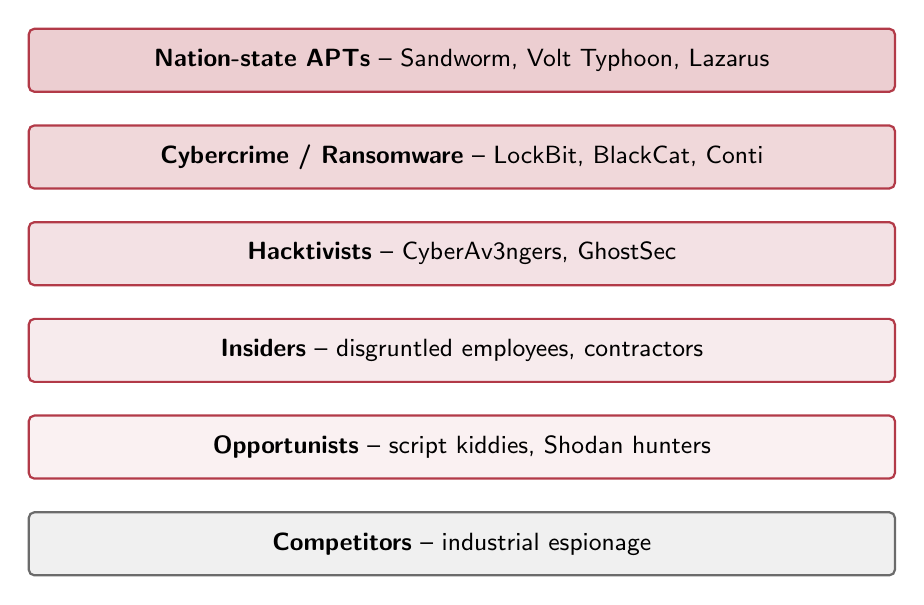
\begin{tikzpicture}[node distance=4mm]
  \node[isbox, fill=isAttack!25, draw=isAttack, minimum width=110mm] (a) {\textbf{Nation-state APTs} -- Sandworm, Volt Typhoon, Lazarus};
  \node[isbox, fill=isAttack!20, draw=isAttack, minimum width=110mm, below=of a] (b) {\textbf{Cybercrime / Ransomware} -- LockBit, BlackCat, Conti};
  \node[isbox, fill=isAttack!15, draw=isAttack, minimum width=110mm, below=of b] (c) {\textbf{Hacktivists} -- CyberAv3ngers, GhostSec};
  \node[isbox, fill=isAttack!10, draw=isAttack, minimum width=110mm, below=of c] (d) {\textbf{Insiders} -- disgruntled employees, contractors};
  \node[isbox, fill=isAttack!7, draw=isAttack, minimum width=110mm, below=of d] (e) {\textbf{Opportunists} -- script kiddies, Shodan hunters};
  \node[isbox, fill=isMute!10, draw=isMute, minimum width=110mm, below=of e] (f) {\textbf{Competitors} -- industrial espionage};
\end{tikzpicture}
\end{frame}

\begin{frame}{MITRE ATT\&CK for ICS Tactics}
\centering
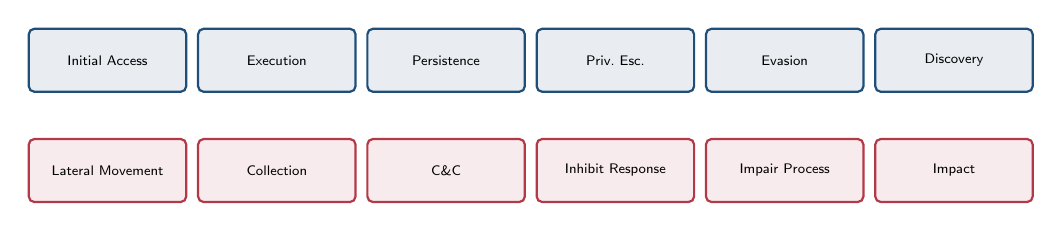
\begin{tikzpicture}[node distance=1.5mm]
  \foreach \i/\name in {
    0/Initial Access,
    1/Execution,
    2/Persistence,
    3/Priv.\ Esc.,
    4/Evasion,
    5/Discovery}{
    \node[isbox, fill=isOT!10, draw=isOT, minimum width=20mm, minimum height=8mm, font=\tiny] (t\i) at ({\i*2.15cm-5.5cm}, 0.7) {\name};
  }
  \foreach \i/\name in {
    0/Lateral Movement,
    1/Collection,
    2/C\&C,
    3/Inhibit Response,
    4/Impair Process,
    5/Impact}{
    \node[isbox, fill=isAttack!10, draw=isAttack, minimum width=20mm, minimum height=8mm, font=\tiny] (b\i) at ({\i*2.15cm-5.5cm}, -0.7) {\name};
  }
\end{tikzpicture}
\par\vspace{3mm}
\begin{notebox}{Why this matters}
ATT\&CK for ICS gives a shared vocabulary for techniques, detections, and incident discussion across teams and vendors.
\end{notebox}
\end{frame}

\section{Landmark Incidents}

\begin{frame}{Stuxnet (2010) -- Kill Chain}
\centering
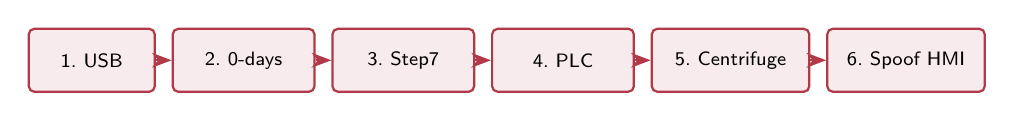
\begin{tikzpicture}[node distance=2mm]
  \node[isbox, fill=isAttack!10, draw=isAttack, minimum width=16mm, font=\scriptsize] (a) {1. USB};
  \node[isbox, fill=isAttack!10, draw=isAttack, right=of a, minimum width=18mm, font=\scriptsize] (b) {2. 0-days};
  \node[isbox, fill=isAttack!10, draw=isAttack, right=of b, minimum width=18mm, font=\scriptsize] (c) {3. Step7};
  \node[isbox, fill=isAttack!10, draw=isAttack, right=of c, minimum width=18mm, font=\scriptsize] (d) {4. PLC};
  \node[isbox, fill=isAttack!10, draw=isAttack, right=of d, minimum width=20mm, font=\scriptsize] (e) {5. Centrifuge};
  \node[isbox, fill=isAttack!10, draw=isAttack, right=of e, minimum width=20mm, font=\scriptsize] (f) {6. Spoof HMI};
  \draw[attack] (a)--(b); \draw[attack] (b)--(c); \draw[attack] (c)--(d);
  \draw[attack] (d)--(e); \draw[attack] (e)--(f);
\end{tikzpicture}
\vspace{1mm}
\begin{notebox}{Natanz, 2010}
Four zero-days, two stolen code-signing certificates. Subtly destroyed an estimated $\sim$1\,000 centrifuges over months while feeding the HMI \emph{normal-looking} data. The first widely-known cyber-physical weapon.
\end{notebox}
\source{N.\ Falliere, L.\ Murchu, E.\ Chien, \emph{W32.Stuxnet Dossier} v1.4, Symantec, 2011 \textbar{} D.\ Albright et al., ISIS report, 2010.}
\end{frame}

\begin{frame}{Ukraine 2015 \& 2016}
\centering
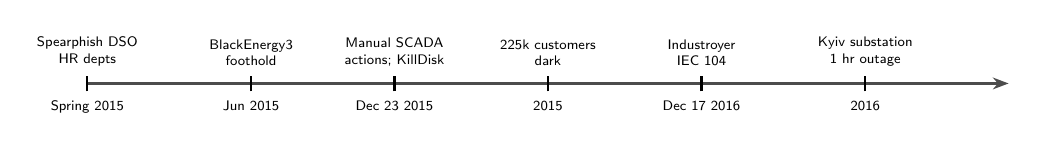
\begin{tikzpicture}[x=1.3cm]
  \draw[axisline] (0,0) -- (9,0);
  \foreach \x/\year/\label in {
    0/{Spring 2015}/{Spearphish DSO\\HR depts},
    1.6/{Jun 2015}/{BlackEnergy3\\foothold},
    3.0/{Dec 23 2015}/{Manual SCADA\\actions; KillDisk},
    4.5/{2015}/{225k customers\\dark},
    6.0/{Dec 17 2016}/{Industroyer\\IEC 104},
    7.6/{2016}/{Kyiv substation\\1 hr outage}}{
    \draw[thick] (\x,-1mm) -- (\x,1mm);
    \node[font=\tiny, below=1mm] at (\x,0) {\year};
    \node[font=\tiny, above=1mm, align=center] at (\x,0) {\label};
  }
\end{tikzpicture}
\par\vspace{3mm}
{\footnotesize Sandworm (GRU). Industroyer was the first malware framework with built-in grid protocol modules.}
\source{R.\ M.\ Lee, M.\ J.\ Assante, T.\ Conway, \emph{Analysis of the Cyber Attack on the Ukrainian Power Grid}, SANS/E-ISAC, 2016 \textbar{} A.\ Cherepanov, \emph{Win32/Industroyer}, ESET, 2017.}
\end{frame}

\begin{frame}{TRITON / TRISIS (2017)}
\centering
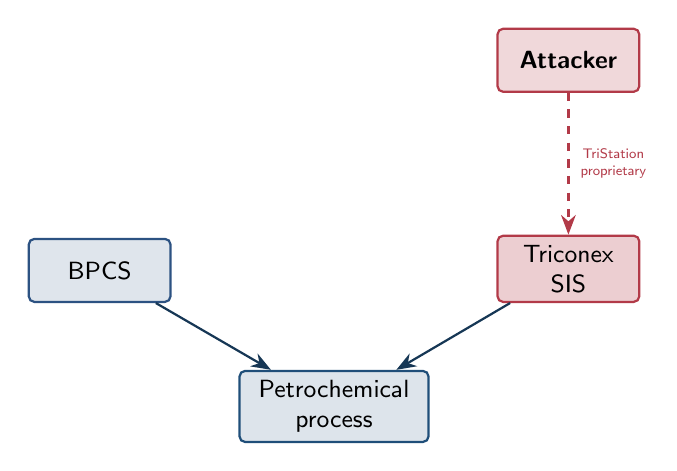
\begin{tikzpicture}[node distance=12mm]
  \node[process] (proc) {Petrochemical\\process};
  \node[plc, above left=of proc] (bpcs) {BPCS};
  \node[plc, above right=of proc, fill=isAttack!25, draw=isAttack] (sis) {Triconex\\SIS};
  \node[attacker, above=18mm of sis] (atk) {Attacker};
  \draw[flow] (bpcs) -- (proc); \draw[flow] (sis) -- (proc);
  \draw[attack] (atk) -- node[right=3pt, font=\tiny, align=center, fill=white, inner sep=1pt]{TriStation\\proprietary} (sis);
\end{tikzpicture}
\par\vspace{1mm}
{\footnotesize First publicly known attack on a Safety Instrumented System. A programming error in the malware tripped the plant and exposed the operation. Watershed moment: attackers reached the safety layer.}
\source{Dragos, \emph{TRISIS Malware Analysis}, 2017 \textbar{} Mandiant/FireEye, \emph{Attackers Deploy New ICS Attack Framework ``TRITON''}, 2017.}
\end{frame}

\begin{frame}{Colonial Pipeline (2021)}
\centering
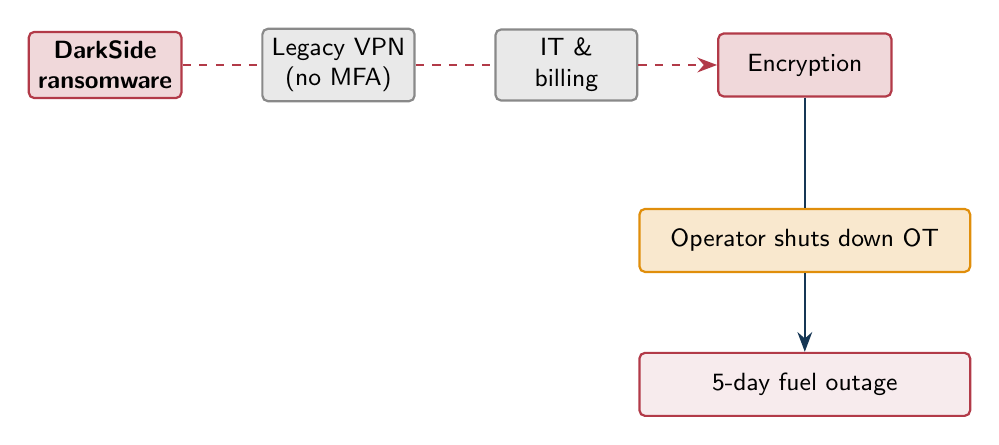
\begin{tikzpicture}[node distance=10mm]
  \node[attacker] (atk) {DarkSide\\ransomware};
  \node[server, right=of atk] (vpn) {Legacy VPN\\(no MFA)};
  \node[server, right=of vpn] (it) {IT \&\\billing};
  \node[isbox, fill=isAttack!20, draw=isAttack, right=of it, minimum width=22mm] (enc) {Encryption};
  \node[isbox, fill=isAccent!20, draw=isAccent, below=14mm of enc, minimum width=42mm] (shut) {Operator shuts down OT};
  \node[isbox, fill=isAttack!10, draw=isAttack, below=of shut, minimum width=42mm] (impact) {5-day fuel outage};
  \draw[attack] (atk) -- (vpn) -- (it) -- (enc);
  \draw[flow] (enc) -- (shut) -- (impact);
\end{tikzpicture}
\par\vspace{1mm}
{\footnotesize IT compromise; the operator pre-emptively halted OT. Highlights IT/OT interdependence and the physical impact of ransomware.}
\source{FBI, \emph{Statement on Colonial Pipeline}, May 2021 \textbar{} GAO-22-104746, 2022.}
\end{frame}

\begin{frame}{CyberAv3ngers / Unitronics (2023)}
\begin{warningbox}{Lessons that keep coming back}
\textbf{Default credentials} and \textbf{direct Internet exposure} of PLCs are still common -- and still get exploited by low-skill actors at scale.
\end{warningbox}
\vspace{1mm}
\centering
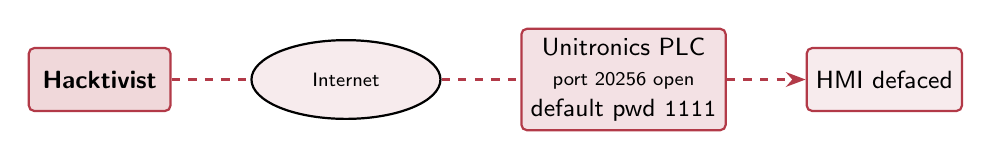
\begin{tikzpicture}[node distance=10mm]
  \node[attacker] (atk) {Hacktivist};
  \node[inetnode, fill=isAttack!10, right=of atk] (inet) {Internet};
  \node[plc, fill=isAttack!15, draw=isAttack, right=of inet] (plc) {Unitronics PLC\\\scriptsize port 20256 open\\default pwd \texttt{1111}};
  \node[isbox, fill=isAttack!10, draw=isAttack, right=of plc] (def) {HMI defaced};
  \draw[attack] (atk) -- (inet) -- (plc) -- (def);
\end{tikzpicture}
\par\vspace{2mm}
{\footnotesize No process damage, but trivially exploited at multiple water utilities. \textbf{Reminder:} never expose OT to the Internet, always change defaults.}
\source{CISA \emph{AA23-335A}, ``IRGC-Affiliated Cyber Actors Exploit PLCs in Multiple Sectors'', 1 Dec 2023.}
\end{frame}

\section{Cross-Cutting Risks}

\begin{frame}{Supply Chain}
\centering
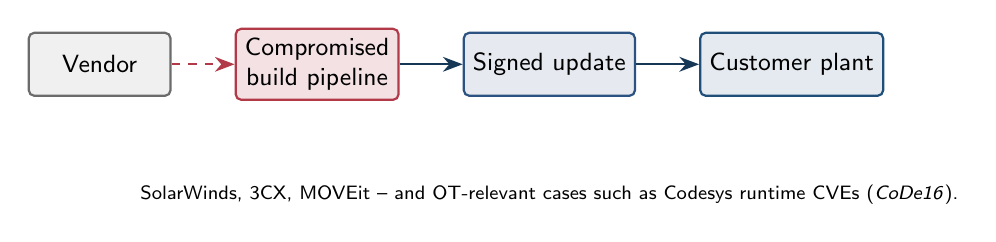
\begin{tikzpicture}[node distance=8mm]
  \node[isbox, fill=isMute!10, draw=isMute] (dev) {Vendor};
  \node[isbox, fill=isAttack!15, draw=isAttack, right=of dev] (cmp) {Compromised\\build pipeline};
  \node[isbox, fill=isPLC!12, draw=isPLC, right=of cmp] (upd) {Signed update};
  \node[isbox, fill=isOT!12, draw=isOT, right=of upd] (cust) {Customer plant};
  \draw[attack] (dev) -- (cmp);
  \draw[flow] (cmp) -- (upd);
  \draw[flow] (upd) -- (cust);
  \node[font=\scriptsize, below=10mm of upd]
    {SolarWinds, 3CX, MOVEit -- and OT-relevant cases such as Codesys runtime CVEs (\emph{CoDe16}).};
\end{tikzpicture}
\end{frame}

\begin{frame}{Insider Threat}
\centering
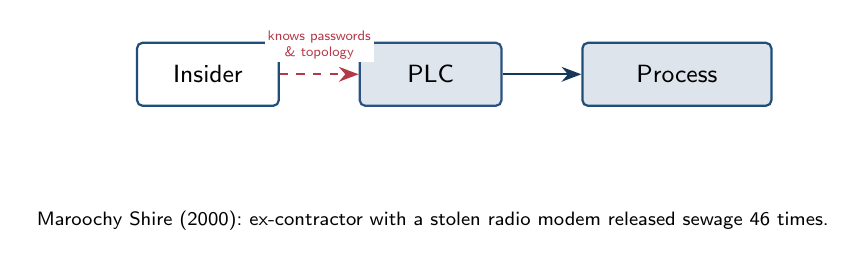
\begin{tikzpicture}[node distance=10mm]
  \node[workstation] (in) {Insider};
  \node[plc, right=of in] (plc) {PLC};
  \node[process, right=of plc] (proc) {Process};
  \draw[attack] (in) -- node[above=4pt, font=\tiny, align=center, fill=white, inner sep=1pt]{knows passwords\\\& topology} (plc);
  \draw[flow] (plc) -- (proc);
  \node[font=\scriptsize, below=12mm of plc, align=center, text width=10cm]
    {Maroochy Shire (2000): ex-contractor with a stolen radio modem released sewage 46 times.};
\end{tikzpicture}
\source{J.\ Slay \& M.\ Miller, ``Lessons learned from the Maroochy Water breach'', \emph{Critical Infrastructure Protection}, IFIP, 2008.}
\end{frame}

\begin{frame}{INCONTROLLER / PIPEDREAM (2022)}
\centering
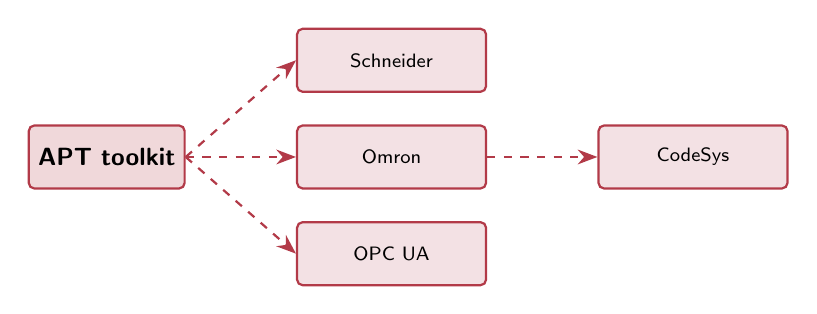
\begin{tikzpicture}[node distance=10mm]
  \node[attacker] (atk) {APT toolkit};
  \node[plc, fill=isAttack!15, draw=isAttack, above right=4mm and 14mm of atk, minimum width=24mm, font=\scriptsize] (s1) {Schneider};
  \node[plc, fill=isAttack!15, draw=isAttack, right=14mm of atk, minimum width=24mm, font=\scriptsize] (om) {Omron};
  \node[plc, fill=isAttack!15, draw=isAttack, below right=4mm and 14mm of atk, minimum width=24mm, font=\scriptsize] (o) {OPC UA};
  \node[plc, fill=isAttack!15, draw=isAttack, right=14mm of om, minimum width=24mm, font=\scriptsize] (cdo) {CodeSys};
  \draw[attack] (atk.east) -- (s1.west);
  \draw[attack] (atk.east) -- (om.west);
  \draw[attack] (atk.east) -- (o.west);
  \draw[attack] (om.east) -- (cdo.west);
\end{tikzpicture}
\vspace{2mm}
\begin{importantbox}{First multi-target ICS framework}
PIPEDREAM is the first modular framework with pre-built modules for several vendors at once -- captured before it was used in anger.
\end{importantbox}
\source{CISA \emph{AA22-103A}, ``APT Cyber Tools Targeting ICS/SCADA Devices'', 13 Apr 2022 \textbar{} Dragos, \emph{PIPEDREAM/CHERNOVITE} report, 2022 \textbar{} Mandiant, \emph{INCONTROLLER}, 2022.}
\end{frame}

\begin{frame}{Volt Typhoon -- Living off the Land in OT}
\begin{itemize}
  \item Suspected China-linked APT, active since at least 2021.
  \item Targets US critical infrastructure: telecoms, water, energy.
  \item Uses \emph{built-in tools} (PowerShell, WMI, native Windows) -- minimal new malware.
  \item Apparent goal: pre-positioning for disruptive action during conflict.
\end{itemize}
\begin{warnbox}
The hardest threat to detect is the one that looks like a normal admin task. Behavioural analytics matter more than signatures.
\end{warnbox}
\source{CISA \emph{AA24-038A}, ``PRC State-Sponsored Actors Compromise and Maintain Persistent Access to U.S.\ Critical Infrastructure'', 7 Feb 2024 \textbar{} Microsoft, \emph{Volt Typhoon}, May 2023.}
\end{frame}

\begin{frame}{Common Initial Access Vectors in ICS}
\centering
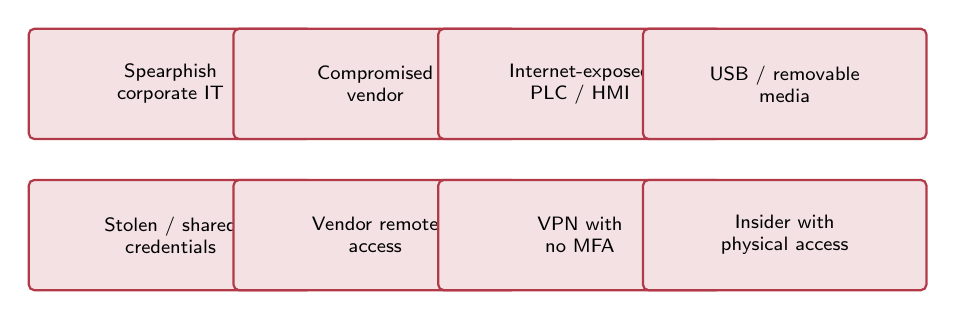
\begin{tikzpicture}[x=2.6cm, y=1.2cm]
  \node[isbox, fill=isAttack!15, draw=isAttack, font=\scriptsize, minimum width=36mm, minimum height=14mm, align=center] at (0,0) {Spearphish\\corporate IT};
  \node[isbox, fill=isAttack!15, draw=isAttack, font=\scriptsize, minimum width=36mm, minimum height=14mm, align=center] at (1,0) {Compromised\\vendor};
  \node[isbox, fill=isAttack!15, draw=isAttack, font=\scriptsize, minimum width=36mm, minimum height=14mm, align=center] at (2,0) {Internet-exposed\\PLC / HMI};
  \node[isbox, fill=isAttack!15, draw=isAttack, font=\scriptsize, minimum width=36mm, minimum height=14mm, align=center] at (3,0) {USB / removable\\media};
  \node[isbox, fill=isAttack!15, draw=isAttack, font=\scriptsize, minimum width=36mm, minimum height=14mm, align=center] at (0,-1.6) {Stolen / shared\\credentials};
  \node[isbox, fill=isAttack!15, draw=isAttack, font=\scriptsize, minimum width=36mm, minimum height=14mm, align=center] at (1,-1.6) {Vendor remote\\access};
  \node[isbox, fill=isAttack!15, draw=isAttack, font=\scriptsize, minimum width=36mm, minimum height=14mm, align=center] at (2,-1.6) {VPN with\\no MFA};
  \node[isbox, fill=isAttack!15, draw=isAttack, font=\scriptsize, minimum width=36mm, minimum height=14mm, align=center] at (3,-1.6) {Insider with\\physical access};
\end{tikzpicture}
\end{frame}

\begin{frame}{Summary -- Section \sectionNumber}
\begin{takeawaybox}{What to remember from this section}
\begin{itemize}\setlength{\itemsep}{2pt}
  \item Threat actors range from script kiddies to nation-state APTs, each with different capabilities.
  \item MITRE ATT\&CK for ICS provides a shared vocabulary for techniques and detections.
  \item Stuxnet $\rightarrow$ Ukraine $\rightarrow$ TRITON shows an escalating willingness to harm.
  \item Supply chain and insider risk demand controls beyond the perimeter.
\end{itemize}
\end{takeawaybox}
\end{frame}

\referencesframe{
  \item Falliere, N., Murchu, L., Chien, E. \emph{W32.Stuxnet Dossier}, v1.4. Symantec, Feb 2011.
  \item Langner, R. \emph{To Kill a Centrifuge}, The Langner Group, Nov 2013.
  \item Albright, D. et al. \emph{Did Stuxnet take out 1{,}000 centrifuges at Natanz?} ISIS, 22 Dec 2010.
  \item Lee, R.M., Assante, M.J., Conway, T. \emph{Analysis of the Cyber Attack on the Ukrainian Power Grid}, SANS/E-ISAC, 18 Mar 2016.
  \item Cherepanov, A. \emph{Win32/Industroyer}, ESET, June 2017.
  \item Dragos. \emph{TRISIS Malware Analysis}, Dec 2017.
  \item Mandiant/FireEye. \emph{Attackers Deploy New ICS Attack Framework ``TRITON''}, Dec 2017.
  \item FBI. \emph{Statement on the Colonial Pipeline attack}, May 2021.
  \item GAO-22-104746. \emph{Critical Infrastructure Protection: Federal Authorities -- Colonial Pipeline Response}, 2022.
  \item CISA \emph{AA22-103A}. ``APT Cyber Tools Targeting ICS/SCADA Devices'' (PIPEDREAM/INCONTROLLER), 13 Apr 2022.
  \item Mandiant. \emph{INCONTROLLER: New State-Sponsored Cyber Attack Tools}, Apr 2022.
  \item Dragos. \emph{PIPEDREAM/CHERNOVITE}, 2022.
  \item CISA \emph{AA23-335A}. ``IRGC-Affiliated Cyber Actors Exploit PLCs in Multiple Sectors'', 1 Dec 2023.
  \item CISA \emph{AA24-038A}. ``PRC State-Sponsored Actors Compromise and Maintain Persistent Access to U.S.\ Critical Infrastructure'' (Volt Typhoon), 7 Feb 2024.
  \item Microsoft Threat Intelligence. \emph{Volt Typhoon targets US critical infrastructure with living-off-the-land techniques}, May 2023.
  \item Slay, J., Miller, M. ``Lessons learned from the Maroochy Water breach.'' In \emph{Critical Infrastructure Protection}, IFIP, 2008.
  \item MITRE. \emph{ATT\&CK for ICS}, knowledge base, \url{https://attack.mitre.org/matrices/ics/}.
  \item Dragos. \emph{Year in Review}, annual reports.
}

\closingframe

\end{document}
